\chapter{Introduction}

\begin{quote}
\emph{This dissertation explores how people use computational notebooks to perform, document, and share data-driven work. It finds a tension between exploration and explanation hinders data analysts from clearly communicating complex analyses, but that computational notebooks can reduce this tension by supporting flexible navigation and organization of analytical components such as executable code, computed results, and explanatory text. This dissertation also explores how computational notebooks might help professionals document and share data-driven work in domains where general-purpose programming is not the primary means of interacting with data. Together these investigations help us understand how computational notebooks and other interactive technologies can help individuals and organizations think with data.}
\end{quote}

\vspace{0.25in}

The cost of collecting, storing, and manipulating data has fallen dramatically over the past 50 years, enabling data to multiply in nearly every sphere of life \cite{reinsel2017data}. Businesses increasingly rely on data about their customers and products to generate value \cite{kandel2012enterprise}. Governments munge data to learn about their constituents and set policy \cite{le2015planning, chicago, nyc}. Scientists collect and model data to study domains as diverse as engineering, the life sciences, and arts. Individuals collect data about their physical activity, spending, and happiness to foster self-awareness \cite{epstein2015lived,li2010stage}. Profits, policy, innovation, and health all increasingly rely on collecting and analyzing data.

But those who understand data are in short supply. McKinsey, a consulting firm, estimates that in 2018 the United States alone will face ``a shortage of 140,000 to 190,000 people with analytical expertise and 1.5 million managers and analysts with the skills to understand and make decisions based on the analysis of big data'' \cite{manyika2011big}. There is an urgent need to both train new analysts and develop tools and techniques that enable them to work more effectively.

Data analysis has been described as simply ``looking at data to see what it seems to say'' \cite{tukey1977exploratory}, but knowing where and how to look is not as simple as it may seem. Insights derived from data are highly dependent on the questions asked and the methods used to inspect them. Two analysts given the same dataset may draw vastly different conclusions \cite{herndon2014does, reinhart2010growth}. Even during analysis, deciding what to do next often requires extensive knowledge of what one has already done with the data and why \cite{gotz2009characterizing, heer2012interactive}. Moreover, the scale of data analyzed today typically requires writing and running numerous small computer programs to collect, clean, and model them. The workings of each of these programs may be difficult to understand in isolation, much less when they are combined. 

These challenges are compounded by the fact that
data analysis is increasingly collaborative \cite{heer_design_2008, kandel2012enterprise}, especially in scientific domains. Even if they work in the same office or field, collaborators may have vastly different skill-sets, terminologies, and goals for an analysis \cite{galison1997image}. Assumptions need to be made explicit and methods explained in detail if data and the insights derived from them are to be clearly communicated \cite{harper1995collaborative}. Those who wish to contribute to open science and publicly share their work face even greater challenges making their analyses legible not just to a particular group of colleagues, but to anyone who might read them. Explaining the exploratory process of data analysis is rarely a straightforward task.

%And there is an explosion of scientific output doubling every nine years. Making one's insights clear amongst the flood of dta and publications is difficult.

\section{The Challenge: Tracking and Sharing Data Analyses}

Data analysts need to keep a detailed record of their analytical steps, reasoning, and results if others are to review, resume, or build on their work.
However, tracking and sharing data analysis is complicated by the number and diversity of steps involved \cite{guo_software_2012, kandel2012enterprise, tabard2008individual} as well as the professional judgment guiding their selection and execution \cite{harper1995collaborative}. 
In the end, most analysts have only incomplete or messy records of their process, especially when their analysis involves programming.

\begin{figure}[t!]%
\centering
\subfigure[]{%
\label{fig:files}%
\frame{
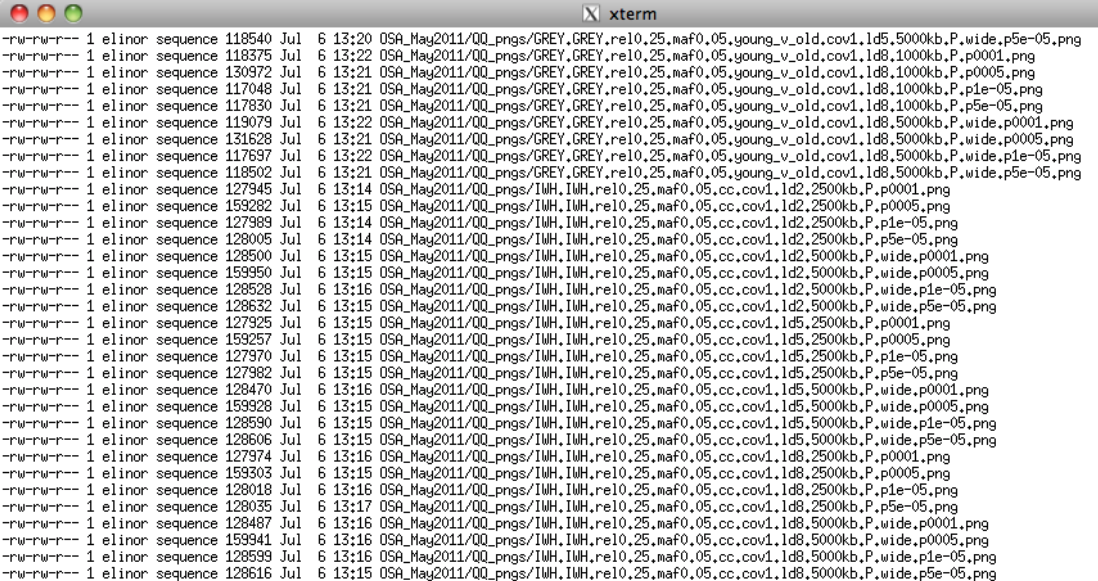
\includegraphics[width=0.9\textwidth]{img/files}}%
}
\quad
\subfigure[]{%
\label{fig:notes}%
\frame{
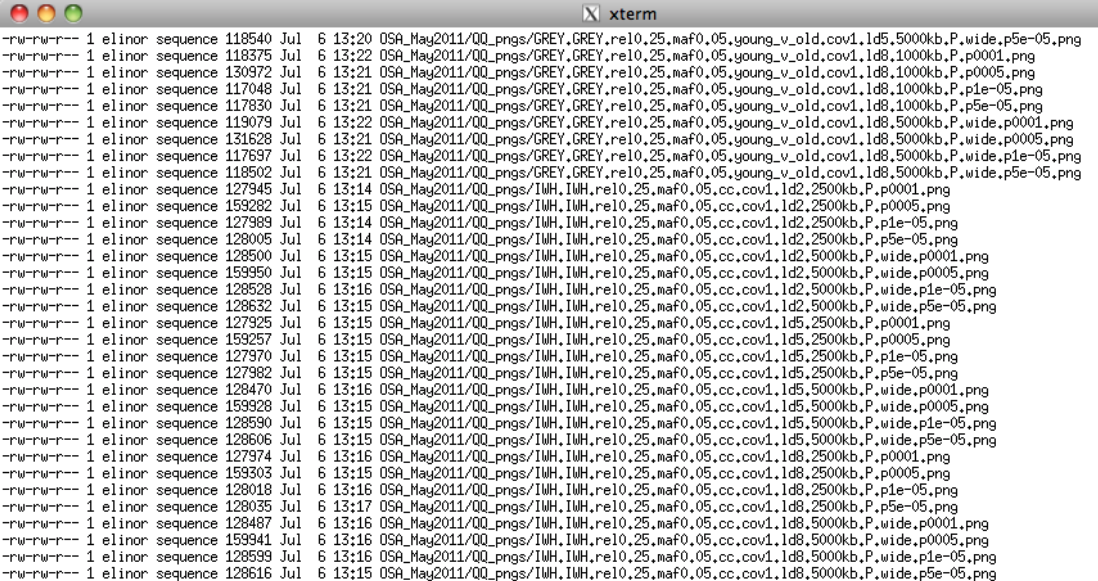
\includegraphics[width=0.9\textwidth]{img/files}}%
}
\caption[Two methods of tracking the process of exploratory data analysis]{Two methods of tracking the process of exploratory data analysis. (a) A partial list of output files for different runs of the same analysis with file names reflecting the parameters of each run, from \cite{guo_software_2012}. (b) A Word document describing a biologist's analytical steps across multiple software tools, from \cite{tabard2008individual}.}
\label{fig:trackmethods}
\end{figure}

Consider Figure \ref{fig:trackmethods} which shows two different methods of tracking data analysis employed by two different biologists. Figure \ref{fig:files} shows a partial list of files in one of the biologist's computer folders \cite{guo_software_2012}. He had run the same analysis script over and over again, tweaking the parameters of the script each time and generating dozens of figures whose similar filenames contain the settings of each run (e.g., ``ld2'' and ``5000kb''). When resuming the analysis after a break, this analyst had difficulty recalling which run had produced the most promising results. Figure \ref{fig:notes} shows a second biologist's attempts to track her analysis \cite{tabard2008individual}. Since she had to manage data across multiple websites and applications she chose to track her steps in a  Word document. Her cryptic notes are a collage of activity: manipulating data from her command line, referencing notes in another notebook, instructions to copy-paste and rerun a step, file paths to yet more data, notes on variations of the analysis with different parameters, and even raw data pasted directly into the Word document itself.

Both methods demonstrate some of the challenge of tracking and sharing data analysis. Iterative analyses tend to produce multiple similar results that take time and energy to document and distinguish. Analyses often require multiple steps across multiple tools, none of which keeps a full record of the process. Manually tracking one's steps is laborious and often produces cryptic notes that even the original analyst has a hard time understanding. In the end neither record is of much use to a collaborator. 

One increasingly popular means of addressing these challenges is to conduct analyses, at least the growing share involving programming, in computational notebooks (Figure \ref{fig:notebook}). These enable analysts to iteratively execute analytical code and interleave it with computed results and explanatory text. Whereas, before, analysts had to copy code and results from various files into a separate report (Figure \ref{fig:notes}), computational notebooks enable them to write, run, and explain their analyses in a single document. In place of large collections of similarly named files (Figure \ref{fig:files}), analysts can combine all explorations in a single annotated document. Computational notebooks have seen widespread adoption in recent years \cite{granger2017jupyterlab} and been hailed by some as a replacement to academic papers as the best vehicle for sharing scientific results. \cite{somers2018scientific}. \emph{Yet, while millions of people use computational notebooks for a variety of data-driven activities, we know little about how they actually use them or how well notebooks address the challenge of tracking and sharing complex data analyses.}

\begin{figure}[b!] 
  \centering
  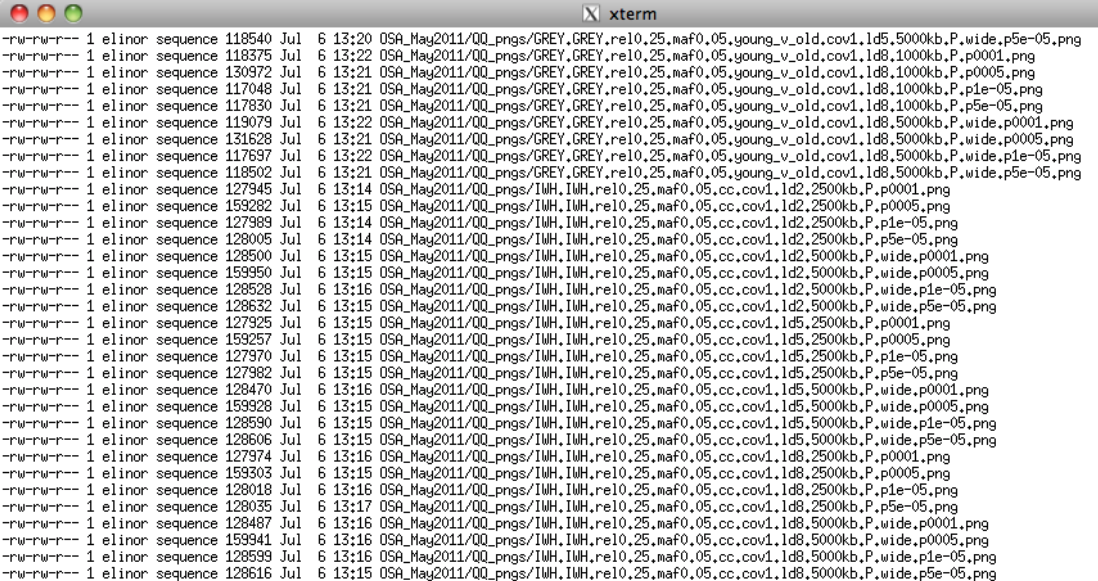
\includegraphics[width=0.93\textwidth]{img/files}
  \caption[A computational notebook]
{A computational notebook combining code, visualizations, text.}
  \label{fig:notebook}
\end{figure}

\section{Thesis}

This dissertation explores challenges analysts face tracking and sharing their data analyses. It focuses on how they currently use computational notebooks to do so, and how these notebooks might be designed to better support their needs. This dissertation also begins to explore how the paradigm of computational notebooks might support data-driven work in domains where programming with a general-purpose programming language is not the primary means of interacting with data, domains such as engineering, healthcare, and government. Underlying these investigations is the thesis:

\begin{quote}
\emph{Understanding how the tension between exploring data and explaining process manifests itself in practice makes it possible to design software that enables analysts to document and share their work more effectively.}
\end{quote}

\section{Contributions}

This dissertation has four types of contributions: empirical results, theoretical perspectives, prototype systems, and an open dataset. Here I summarize these contributions in the order they will be presented in the chapters that follow (Figure \ref{fig:contributions}).

\begin{figure}[t!] 
  \centering
    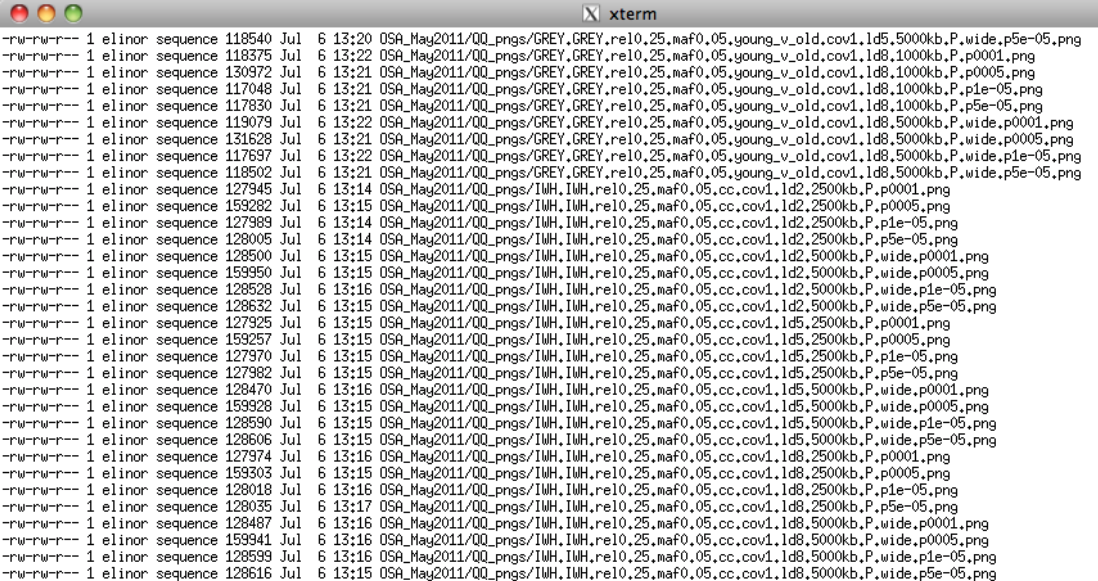
\includegraphics[width=1.0\textwidth]{img/files}
  \caption[Contributions of this dissertation]
{Contributions of this dissertation including empirical results, prototype systems, theoretical perspectives, and an open dataset.}
  \label{fig:contributions}
\end{figure}

\textsc{Chapter 3} presents three studies characterizing the use of \emph{computational narrative} (i.e., the interleaving of code and visualizations with explanatory text) in computational notebooks. In the first study I analyze over 1 million Jupyter Notebooks hosted publicly on GitHub, finding that more than a quarter lack even a single word of explanatory text. Even those notebooks that had explanatory text were mostly loose collections of notes and scripts without a coherent structure. In a second study I systematically code over 200 notebooks supplementing academic publications, finding that even when these notebooks have explanatory text, only about a third use that text to discuss analytical reasoning or to interpret results. Even among these academic notebooks where we might expect authors to include detailed explanations of their work to support future research, most authors used explanatory text to simply label the steps of their analysis. In a third study I interview 15 academic data analysts, finding that this lack of narrative stems from the tendency for exploratory analyses to produce messy notebooks that are difficult to understand. Cleaning and sharing these notebooks takes more effort than copying a final figure into an email, which may be all that analysts feel their collaborators want to see.

Together these findings support a theoretical perspective that a tension between exploration and explanation makes it difficult to track and share data analyses, regardless of the medium involved. The iterative and messy process of exploring data is fundamentally at odds with the careful, reflective process of explaining what the results of those explorations mean. In addition to these empirical findings and theoretical perspective, I also released all data from the first study, including over a million computational notebooks, as a single dataset for others to download and study (\url{https://doi.org/10.6075/J0JW8C39}).

In \textsc{Chapter 4} I build on these findings by exploring how computational notebooks might be redesigned to encourage clearer communication of complex data analyses, in particular by including more explanatory text and explicit organization. Taking the point-of-view that notebooks need to provide an immediate benefit to organization and annotation activities I design and develop Janus, a Jupyter Notebook extension that enables analysts to add history and hierarchy to their notebooks. Through two studies, the first a formative study with novice analysts and the second a multi-week technology probe with expert analysts, I demonstrate that hierarchy in particular enables analysts to flexibly organize and navigate their notebooks in ways that support both the ongoing analysis and later communication of results. These findings support the theoretical perspective that flexible organization and navigation of code, visualizations, and text can help reduce the tension between exploration and explanation by providing a lightweight and fast way to tailor notebooks to the task at hand.

In \textsc{Chapter 5} I explore how the the paradigm of computational notebooks might support data-driven work in a domain where general-purpose programming in not the primary means of interacting with data. With a team of collaborators I helped design and test ActiveNotes, a prototype clinical note editor that enables clinicians to place medication orders while typing free-text notes. This work provides empirical results about how clinicians might use free-text order entry, and supports the theoretical perspective that notebooks mixing free-text and commands written in a domain-specific language might support data-driven work outside traditional data analysis.

Together these investigations help us understand how computational notebooks and other interactive media might help individuals and organizations think with data.
